% Appendix A

\chapter{Option contracts} % Main appendix title

\label{AppendixA} % For referencing this appendix elsewhere, use \ref{AppendixA}

This list of option contracts are far from complete, but the purpose is to illustate some payoff contracts for reference.

\section{European Call and Put}
The European options will be the most basic options, we will work with. This means not that they are not important, actually they are key for pricing options. The European call option is a contract, which pays at maturity $\Phi(S(T))=max(S-K,0)$. 
\begin{figure}[h]
\centering
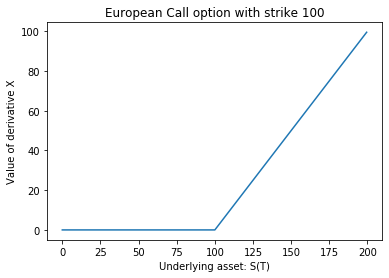
\includegraphics{Figures/euroCall.png}
\decoRule
\caption[]{European call with K=100}
\label{fig:EuroCall}
\end{figure}

The European put is very similar to the call, except now we earn, when the stock is below the strike price K.\\
$\Phi(S(T))=max(K-S,0)$.
\begin{figure}[h]
\centering
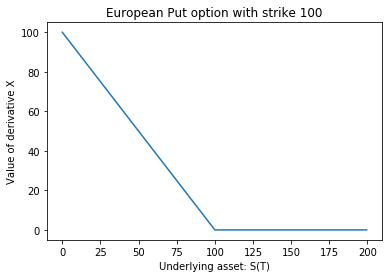
\includegraphics{Figures/euroPut.png}
\decoRule
\caption[]{European put with K=100}
\label{fig:EuroPut}
\end{figure}